\documentclass[
	article,		
	11pt,			
	oneside,		
	a4paper,			
	english,			
	brazil			
]{abntex2}

\usepackage{lmodern}		
\usepackage[T1]{fontenc}		
\usepackage[utf8]{inputenc}		
\usepackage{indentfirst}		
\usepackage{nomencl} 			
\usepackage{color}				
\usepackage{graphicx}		
\usepackage{microtype} 		
\usepackage[brazilian]{backref}
\usepackage[alf]{abntex2cite}
\usepackage{makecell}

\definecolor{blue}{RGB}{41,5,195}

\makeatletter
\hypersetup{
		pdftitle={\@title}, 
		pdfauthor={\@author},
    	pdfsubject={Modelo de artigo científico com abnTeX2},
	    pdfcreator={LaTeX with abnTeX2},
		pdfkeywords={abnt}{latex}{abntex}{abntex2}{atigo científico}, 
		colorlinks=true,       		
    	linkcolor=blue,          	
    	citecolor=blue,        		
    	filecolor=magenta,      	
		urlcolor=blue,
		bookmarksdepth=4
}

\makeatother
\makeindex

\setlrmarginsandblock{3cm}{3cm}{*}
\setulmarginsandblock{3cm}{3cm}{*}
\checkandfixthelayout
\setlength{\parindent}{1.3cm}
\setlength{\parskip}{0.2cm}

\SingleSpacing
\frenchspacing 

\begin{document}
\selectlanguage{brazil}
\titulo{Bel, Decibel e sua importância para o estudo do som}
\tituloestrangeiro{Bel, Decibel and its importance for the study of sound}
\autor{Pedro Oliveira Sousa}
\maketitle

\begin{resumoumacoluna}
Intensidade do som é a quantidade de energia que as ondas sonoras transferem, através de uma área, durante o intervalo de tempo de um segundo. Ela é usada para medir o fluxo de energia que é transportado por uma onda sonora. De acordo com o Sistema Internacional de Unidades, a intensidade do som é medida em unidades de W/m².

É provável que você já tenha ouvido falar sobre decibels (dB). Essa medida de intensidade sonora é usada para se comparar a intensidade de diferentes sons (de mesma frequência). O decibel é uma unidade derivada do bel (B), que é uma escala logarítmica que compara a intensidade de um som com a menor intensidade de som que pode ser observada pelo ser humano. Frequentemente a escala de bel é expressa em décimos de sua unidade, chamados de decibels.\cite{HELERBROCKIntensidadeSomBrasilEscola}

\vspace{\onelineskip}
\noindent
\textbf{Palavras-chaves:}
\begin{enumerate}
    \item Intensidade do som 
    \item Bel
    \item Decibels
    \item Escala logarítima
\end{enumerate}
\end{resumoumacoluna}

\renewcommand{\resumoname}{Abstract}
\begin{resumoumacoluna}
Sound intensity is the amount of energy that sound waves transfer through an area during a time interval of one second. It is used to measure the flow of energy that is carried by a sound wave. According to the International System of Units, sound intensity is measured in units of W/m².

You've probably heard about decibels (dB). This measure of sound intensity is used to compare the intensity of different sounds (of the same frequency). The decibel is a unit derived from the bel (B), which is a logarithmic scale that compares the intensity of a sound with the lowest intensity of sound that can be observed by a human being. The bel scale is often expressed in tenths of its unit, called decibels.\cite{HELERBROCKIntensidadeSomBrasilEscola}

\vspace{\onelineskip}
\noindent
\textbf{Key-words:}
\begin{enumerate}
    \item Sound intensity 
    \item Bel
    \item Decibels
    \item Logarithmic scale
\end{enumerate}
\end{resumoumacoluna}

\textual

\section{Introdução}

O decibel (dB) é uma unidade usada para medir a intensidade do som e outras grandezas físicas. Um decibel é um décimo de um bel (B), uma unidade com o nome de Graham Bell, o inventor do telefone. Sua escala logarítmica é adequada para representar o espectro auditivo do ser humano.

\section{Discussão}

\subsection{Intensidade}
Os sons apresentam três características – intensidade, altura e timbre. Intensidade, timbre e altura são características, ou propriedades dos sons. A intensidade sonora refere-se à potência da fonte emissora, bem como à quantidade de energia que o som é capaz de transportar; o timbre diz respeito ao formato das oscilações sonoras e a altura, por sua vez, é determinada pela frequência do som.

Quando algum som tem grande intensidade, dizemos que esse som é forte, ao contrário, trata-se de um som fraco. É esta propriedade do som que nos permite distinguir uma fonte sonora de outra, apesar de estarem a produzir sons com a mesma frequência e intensidade. Projeto Educação: veja questão resolvida sobre cálculo de intensidade sonora

A intensidade das ondas sonoras é proporcional à amplitude da onda sonora, e não à sua frequência, por isso dizemos que sons de grande intensidade são sons fortes, enquanto sons de baixa intensidade são chamados de sons fracos. Sons de grande intensidade são capazes de transferir grandes quantidades de energia a cada segundo, podendo causar danos à audição, por exemplo.\cite{HELERBROCKIntensidadeSomBrasilEscola}

A intensidade sonora mede a quantidade de energia que uma onda sonora é capaz de transferir a cada segundo em uma área de 1 m². A intensidade relaciona-se à amplitude da onda e é definida pela potência emitida pela fonte dividida pela área da frente de onda sonora, como mostramos a seguir:

\begin{equation}
    I=\frac{P}{A}
\end{equation}

\begin{center}
I - Intensidade sonora (W/m²)\\
P - Potência (W)\\
A - Área da frente de onda (m²)
\end{center}

A figura a seguir ilustra a frente de onda sonora, que tem formato circular, uma vez que as sonoras são tridimensionais e propagam-se com a mesma velocidade em todas as direções:
\begin{figure}[h]
    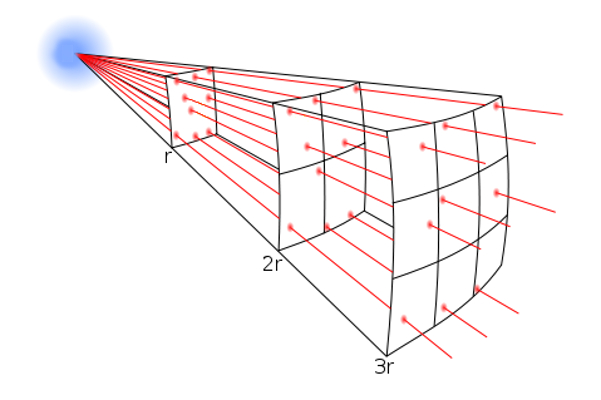
\includegraphics[width=0.80\textwidth]{./imagens/intensidade-do-som-e-distancia-2.jpg}
    \centering
    \caption{A intensidade sonora diminui com o quadrado da distância entre a fonte e o observador.}
    \label{fig:Intencidade sonora}
\end{figure}

Por meio da figura, é possível perceber que, conforme nos afastamos uma distância r, a área da frente de onda aumenta com o quadrado da distância. Por tratar-se de uma onda esférica, essa área pode ser calculada pela expressão $4 \cdot \pi^2$.

Apesar de a unidade de intensidade sonora ser o watt por metro quadrado, a intensidade sonora é comumente medida em uma escala logarítmica conhecida como escala de Bell, criada pelo inventor do telefone, Alexander Graham Bell.

A escala de Bell utiliza as propriedades do logaritmo de base 10 para comparar sons de diferentes intensidades, para tanto, o menor valor existente nessa escala é também o menor valor de intensidade sonora audível (chamada de I0), cerca de 10-12 W/m², também conhecido como limiar de audibilidade. De acordo com essa escala, sons de diferentes intensidades relacionam-se com I0 da seguinte maneira:

\begin{equation}
    I = I_0 \cdot 10^N
\end{equation}

\begin{center}
N - Número de bel
\end{center}

Aplicando as propriedades logarítmicas na equação apresentada, obtém-se a seguinte expressão:

\begin{equation}
    N(dB) = 10 \cdot log_{10} (\frac{I}{I_0}) \rightarrow I_0 = 10^{-12} W/m^2
\end{equation}

O cálculo acima permite calcular o número de decibéis de uma onda sonora de intensidade I. O decibel é um submúltiplo dez vezes menor que o bel. A partir disso, é possível compreender que um som de 20 decibéis é 10 vezes mais forte que um som de 10 decibéis, por exemplo.

Quando algum som tem grande intensidade, dizemos que esse som é forte, ao contrário, trata-se de um som fraco.

\subsection{Timbre}

\begin{figure}[h]
    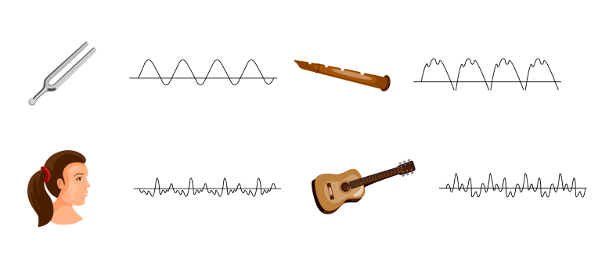
\includegraphics[width=0.80\textwidth]{./imagens/timbre.jpg}
    \centering
    \caption{O timbre permite distinguirmos diferentes fontes sonoras graças ao formato da onda.}
    \label{fig:Timbre}
\end{figure}

O timbre é a característica dos sons que nos permite diferenciar uma nota musical emitida por um piano de um violino, por exemplo. O timbre é o formato da onda sonora, cada instrumento musical apresenta um modo de vibração próprio, que resulta na produção de um som característico.

O timbre também garante que a voz humana seja diferente em cada indivíduo, permitindo que ativemos dispositivos por meio de comandos de voz, por exemplo.

\subsection{Altura}

\begin{figure}[h]
    
\includegraphics[width=0.80\textwidth]{./imagens/caracateristicas-dos-sons.jpg}
    \centering
    \caption{Os sons apresentam três características – intensidade, altura e timbre.}
    \label{fig:CaracteriasticaDoSom}
\end{figure}

A altura de um som diz respeito à sua frequência, que mede o número de oscilações que a onda sonora produz a cada segundo. A medida de frequência é dada em hertz (Hz).

\begin{equation}
    f = \frac{n}{\Delta t}
\end{equation}

\begin{center}
    n – número de oscilações\\
    {$\Delta$} t – intervalo de tempo (s)
\end{center}

A frequência do som pode ser obtida por meio da velocidade de propagação e do comprimento de onda do som. Observe:

\begin{equation}
    V = \lambda f \rightarrow f = \frac{V}{\lambda}
\end{equation}

\begin{center}
    v – velocidade de propagação (m/s)\\
    $\lambda$ – comprimento de onda (m)\\
    f – frequência (Hz)
\end{center}

Os seres humanos não são capazes de ouvir qualquer frequência sonora, na verdade, a nossa percepção é bastante limitada: só somos capazes de ouvir frequências que se encontrem em intervalo que vai de 20 Hz a 20.000 Hz, esse intervalo é conhecido como espectro audível.

Qualquer som que tenha frequência abaixo dos 20 Hz é inaudível pelos seres humanos e é chamado de infrassom, já os sons que tenham frequência maior que 20.000 Hz, também inaudíveis para nós, são conhecidos como ultrassons. Quer saber mais sobre o assunto? Acesse o nosso texto sobre infrassons e ultrassons.

Confira a tabela mostrada a seguir, que relaciona a intensidade sonora com os possíveis efeitos negativos à saúde humana. Os dados exibidos estão de acordo com as diretrizes da Organização Mundial da Saúde (OMS):
\newpage
\input{./tabela}


\section{Considerações Finais}

O bel é utilizado para exprimir o valor de grandeza logarítmicas como o nível de campo, de potência, de intensidade sonora, de pressão acústica ou de atenuação. Os logaritmos de base dez são utilizados para se obterem os valores numéricos das grandezas expressas em bel. Como as medidas de intensidadesonora caracterizam números muito pequenos, usamos uma medida que as relaciona com o menor som que pode ser ouvido pelos seres humanos. Essa medida é conhecida como bel. Essa medida logarítmica foi nomeada em homenagem ao inventor estadunidense Alexander Graham Bell.
Cada intensidade sonora é associada a um “nível de intensidade sonora”. Intensidade e nível de intensidade não devem ser confundidos. A unidade de nível de intensidade sonora é o “decibel”. Como o leitor já desconfia, o símbolo do decibel é “dB”. Por definição do Bell Labs, 1 Bel é igual a atenuação em um sinal de áudio em uma milha (1,61 km) de cabo telefônico.

A intensidade das ondas sonoras é proporcional à amplitude da onda sonora, e não à sua frequência, por isso dizemos que sons de grande intensidade são sons fortes, enquanto sons de baixa intensidade são chamados de sons fracos. Sons de grande intensidade são capazes de transferir grandes quantidades de energia a cada segundo, podendo causar danos à audição, por exemplo.

\bookmarksetup{startatroot}

\bibliography{Ref2.bib}

\end{document}
